\documentclass[final,12pt,a4paper]{COMP4910}

\usepackage[turkish]{babel}
\usepackage[utf8]{inputenc}

\usepackage[english]{babel}
\usepackage[latin5]{inputenc}

\usepackage{caption}
\usepackage{listings}
\lstset{
	literate={~} {$\sim$}{1}, % set tilde as a literal (no process)      % the language of the code
	basicstyle=\ttfamily\fontsize{7}{8}\selectfont\bfseries,
	frame=tb,
	linewidth=0.98\linewidth,
	columns=flexible,
	numbers=left,                   % where to put the line-numbers
	stepnumber=1,                   % the step between two line-numbers. If it's 1, each line will be numbered
	numbersep=5pt,                  % how far the line-numbers are from the code
	showspaces=false,               % show spaces adding particular underscores
	showstringspaces=false,         % underline spaces within strings
	showtabs=false,                 % show tabs within strings adding particular underscores
	frame=single,                   % adds a frame around the code
	tabsize=2,                      % sets default tabsize to 2 spaces
	captionpos=b,                   % sets the caption-position to bottom
	breaklines=true,                % sets automatic line breaking
	breakatwhitespace=false,        % sets if automatic breaks should only happen at whitespace
	caption=\lstname,                 % show the filename of files included with \lstinputlisting; also try caption instead of title
	escapeinside={\%*}{*)},            % if you want to add a comment within your code
	morekeywords={*,...},               % if you want to add more keywords to the set
	lineskip={-1.2pt},
}

\usepackage{latexsym}
\usepackage{amsfonts}
\usepackage{amssymb}
\usepackage{fancyhdr}
\usepackage{setspace}
\usepackage{multicol}

\usepackage{amsmath}

\usepackage[linesnumbered,ruled]{algorithm2e}
\DontPrintSemicolon
\SetKwInOut{Input}{input}
\SetKwInOut{Output}{output}
\usepackage{setspace}
\usepackage{etoolbox}
\AtBeginEnvironment{algorithm}{\setstretch{1.15}}
\SetKwInOut{Input}{Input}
\SetKwInOut{Output}{Output}

\usepackage{float}
\floatstyle{ruled}
\usepackage{graphicx}
\graphicspath{{figures/}}
\newfloat{myfigure}{thp}{lop}
\floatname{myfigure}{Figure}
\newfloat{mytable}{thp}{lop}
\floatname{mytable}{Table}
\usepackage{multicol}
\usepackage{mathtools}
\DeclarePairedDelimiter\ceil{\lceil}{\rceil}
\DeclarePairedDelimiter\floor{\lfloor}{\rfloor} %usage \floor*{2/3}

\usepackage{enumerate}
\usepackage{latexsym}
\usepackage{graphicx}
\usepackage{amsfonts}
\usepackage{amssymb}
\usepackage{fancyhdr}
\usepackage{setspace}
\usepackage{float}
\usepackage{multicol}
\usepackage{color,soul}
\usepackage{url}
\usepackage{tocloft}
\usepackage{acro}

\usepackage{hyperref}
\hypersetup{%
    pdfborder = {0 0 0},
    colorlinks,
    citecolor=,
    filecolor=,
    linkcolor=,
    urlcolor=
} 
\urlstyle{same}


\usepackage{amsthm}
\newtheorem{theorem}{Theorem}[section]
\newtheorem{corollary}{Corollary}[theorem]
\newtheorem{lemma}[theorem]{Lemma}
\newtheorem{remark}[theorem]{Remark}

\linespread{1.5}
\usepackage{helvet}
\renewcommand{\familydefault}{\sfdefault}
\renewcommand{\rmdefault}{phv} % Arial
\renewcommand{\sfdefault}{phv} % Arial

%Remove chapter numbers from sections.
%\renewcommand*\thesection{\arabic{section}}
\renewcommand*\contentsname{\large{TABLE OF CONTENTS}}
\renewcommand*\listtablename{\large{LIST OF TABLES}}
\renewcommand*\listfigurename{\large{LIST OF FIGURES}}
\renewcommand*\listalgorithmcfname{\large{LIST OF ALGORITHMS}}
\renewcommand*\algorithmcfname{Algorithm}
\renewcommand*\algorithmautorefname{algorithm}
\renewcommand*\lstlistingname{Code}
\renewcommand*\lstlistlistingname{LIST OF CODES}
\DeclareCaptionType{code}[Code Listing][\large{LIST OF CODES}] 

\addto\captionsenglish{\renewcommand{\figurename}{Figure}}
\addto\captionsenglish{\renewcommand{\tablename}{Table}}
\addto\captionsenglish{\renewcommand{\bibname}{References}}
\tolerance=10000
\hyphenpenalty=5000

\university{YASAR UNIVERSTIY}
\faculty{FACULTY OF ENGINEERING}
\dept{DEPARTMENT OF COMPUTER ENGINEERING}
\course{COMP4910 Senior Design Project 1, Fall 2019}
\advisor{\large{Supervisor}: {Mutlu BEYAZIT}}
\title{{Project Code Name}: {SLATE}}
\date{{28.12.2019}}
%\submitted{Izmir, 2017} %This field has been disabled Do not use it.

\author{
	{Tuna ALAYGUT}, Student ID: {15070001002}\\
	{Berkay BAYINDIR}, Student ID: {16070001002}\\
	{Alara İŞCAN}, Student ID: {15070001016}\\
}


\revision{Revision\,1.0}
%\revision{Revision\,2.0}
\revision{Final Report}


\dedication{
	\hl{You can dedicate your thesis.}
}

\acknowledgements{
	{The acknowledgements are here.}
}

\keywords{ 
	{convolutional neural network, sign language interpretation, computer vision}
}

\abstract{
	{Slate, is a project designed to facilitate the daily communication of speech/hearing impaired. Fundamentally, it consists of three main components. First component is an external display which is capable of working with a generic smartphone and is located at the back of the smartphone. Second component, in the heart of Slate, is an artificial intelligence which detects, segmentates and classifies hand gestures in the sign language alphabet. Third component is a smart phone application which is resposible for communicating the artificial intelligence and external display components. It also provides an interface to the users of the project.\\Artificial intelligence component does the reading the hand gestures from smartphone camera, classification of the gesture and the application component transfers it to the external display. Making it easier for speech/hearing impaired to engage in daily conversations. Slate, acts as an interpreter in these conversations.}
}

\ozet{
	{Slate, işitme/konuşma engelli, işaret dili kullanan kişilerin günlük hayattaki iletişimlerini kolaylaştırmaya yönelik tasarlanan bir projedir. Temelde üç bileşenden oluşmaktadır. Bu bileşenlerden ilki akıllı telefonlar ile birlikte çalışabilen, telefonun arkasında konumlandırılacak bir dış ekran ünitesidir. İkinci bileşen ise projenin merkezinde bulunan, işaret dili alfabesini tanıyıp, sınıflandırıp, yazıya çeviren bir yapay zeka bileşenidir. Üçüncü ve son bileşen ise ilk iki bileşenin iletişiminden sorumlu olan ve kullanım kolaylığı sağlayan akıllı telefon uygulamasıdır.\\ Yapay zeka bileşini, akıllı telefonun kamerasından aldığı ve yazıya dönüştürdüğü işaret dili karakterlerini dış ekran ünitesine yollar. Böylece işaret dili kullanan kişilerin, karşılarındaki kişiler ile iletişimi sağlanmış olur. Slate bu iletişimde bir tercüman rolü oynar.}
}


\DeclareAcronym{GCD}{
	short = \hl{GCD},
	long  = \hl{Greatest Common Divisor},
}

\DeclareAcronym{ECC}{
	short = \hl{ECC},
	long  = \hl{Elliptic Curve Cryptography},
}






\begin{document}
	\chapter{INTRODUCTION}\label{ch:Introduction}
	{Slate is a bla bla.}



\section{Description of the Problem}

\begin{itemize}
	\item \hl{Give an overview of the problem area and your specific problem that you aim to solve.}
	\item \hl{If necessary, provide a literature survey, that is who has done what in this specific problem area, with references to bibliographic resources.}
	\item \hl{If there already exists a number of solutions/products related to your specific problem, present a comparative evaluation of these solutions/products.}
	\item \hl{State that a detailed description of the problem is provided in Appendix A: Requirement Specifications Document.}
\end{itemize}


\section{Project Goal(s)}

\begin{itemize}
	\item \hl{Goal(s) of your project}
	\item \hl{Basically extracted from Section 1.1 of this report.}
	\item \hl{For example: ``To develop a prototype, a model, a software product, a hardware product, a hardware/software product, a process, etc. in \ldots''}
\end{itemize}

\section{Project Output(s)}

\begin{itemize}
	\item \hl{Give a list of all project outputs for COMP 4910.}
	\item \hl{Also, provide a list of predicted additional outputs for COMP 4920.}
	\item \hl{When completed, your project outputs are a software product or a hardware product or a hardware/software product, with all the associated documents such as RSD's, DSD's and PM.}
\end{itemize}


\section{Project Activities and Schedule}


\begin{itemize}
	\item \hl{Your activities and schedule for COMP 4910 activities}
	\item \hl{Also, your planned activities and schedule for COMP 4920 activities}
	\item \hl{For example: Produce first version of problem definition, our 4910 project assignment form, then produce RSD v1.0, then DSD v1.0 as high level design, then DSD v2.0 as detailed design, then implementation and testing activities, then PM, etc}
\end{itemize}



	\chapter{DESIGN}\label{ch:Design}
	\hl{An introductory text for your design goes here.}


%%%%%%%%%%%%%%%%%%%%%%%%%%%%%%%%%%%%%%%%%%%%%%%%%%%%%%%%%%
%%%%%%%%%%%%%%%%%%%%%%%%%%%%%%%%%%%%%%%%%%%%%%%%%%%%%%%%%%
%%%%%%%%%%%%%%%%%%%%%%%%%%%%%%%%%%%%%%%%%%%%%%%%%%%%%%%%%%
\section{High Level Design}

\begin{itemize}
	\item \hl{Describe what you have done as high level design.}
	\item \hl{State that your high level design is provided in Appendix B: Design Specifications Document by referring to its relevant sections. Of course, you should place your high level design into the referenced sections of this appendix properly.}
\end{itemize}


%%%%%%%%%%%%%%%%%%%%%%%%%%%%%%%%%%%%%%%%%%%%%%%%%%%%%%%%%%
%%%%%%%%%%%%%%%%%%%%%%%%%%%%%%%%%%%%%%%%%%%%%%%%%%%%%%%%%%
%%%%%%%%%%%%%%%%%%%%%%%%%%%%%%%%%%%%%%%%%%%%%%%%%%%%%%%%%%
\section{Detailed Design}

\begin{itemize}
	\item \hl{Describe your plan to detail your high level design in COMP4920.}
	\item \hl{This section will be completed in COMP 4920.}
\end{itemize}


\ac{GCD} is an acronym.

%%%%%%%%%%%%%%%%%%%%%%%%%%%%%%%%%%%%%%%%%%%%%%%%%%%%%%%%%%
%%%%%%%%%%%%%%%%%%%%%%%%%%%%%%%%%%%%%%%%%%%%%%%%%%%%%%%%%%
%%%%%%%%%%%%%%%%%%%%%%%%%%%%%%%%%%%%%%%%%%%%%%%%%%%%%%%%%%
\section{Realistic Restrictions and Conditions in the Design}

\begin{itemize}
	\item \hl{Describe restrictions and conditions in your design.}
	\item \hl{For example: No security, limited password enforcement, serves only up to 1000 users simultaneously, does not support distributed files, etc.}
	\item \hl{If you have already written about your design decisions related to restrictions and conditions in your design in detail, you should make a summary here and refer to the related sections.}
\end{itemize}


	\chapter{IMPLEMENTATION, TESTS and TEST DISCUSSIONS}\label{ch:Implementation}
	\hl{An introductory text for your implementation goes here.}


%%%%%%%%%%%%%%%%%%%%%%%%%%%%%%%%%%%%%%%%%%%%%%%%%%%%%%%%%%
%%%%%%%%%%%%%%%%%%%%%%%%%%%%%%%%%%%%%%%%%%%%%%%%%%%%%%%%%%
%%%%%%%%%%%%%%%%%%%%%%%%%%%%%%%%%%%%%%%%%%%%%%%%%%%%%%%%%%
\section{Implementation of the Product}

\begin{itemize}
	\item \hl{Discuss techniques, tools, technologies, etc. that you have considered so far to realize the product in COMP 4920.}
	\item \hl{This section will be completed in COMP 4920.}
\end{itemize}




%%%%%%%%%%%%%%%%%%%%%%%%%%%%%%%%%%%%%%%%%%%%%%%%%%%%%%%%%%
%%%%%%%%%%%%%%%%%%%%%%%%%%%%%%%%%%%%%%%%%%%%%%%%%%%%%%%%%%
%%%%%%%%%%%%%%%%%%%%%%%%%%%%%%%%%%%%%%%%%%%%%%%%%%%%%%%%%%
\section{Tests and Results of Tests}

\begin{itemize}
	\item \hl{Discuss what you have considered so far on how to test your product in COMP 4920.}
	\item \hl{This section will be completed in COMP 4920.}
\end{itemize}


\ac{GCD} is an acronym.


	\chapter{CONCLUSIONS}\label{ch:Conclusion}
	\hl{A conc�usion text for your project goes here.}


%%%%%%%%%%%%%%%%%%%%%%%%%%%%%%%%%%%%%%%%%%%%%%%%%%%%%%%%%%
%%%%%%%%%%%%%%%%%%%%%%%%%%%%%%%%%%%%%%%%%%%%%%%%%%%%%%%%%%
%%%%%%%%%%%%%%%%%%%%%%%%%%%%%%%%%%%%%%%%%%%%%%%%%%%%%%%%%%
\section{Summary}

\begin{itemize}
	\item \hl{Summary of your project}
	\item \hl{Discuss what you have done so far.}
\end{itemize}

\ac{ECC} is an acronym.


%%%%%%%%%%%%%%%%%%%%%%%%%%%%%%%%%%%%%%%%%%%%%%%%%%%%%%%%%%
%%%%%%%%%%%%%%%%%%%%%%%%%%%%%%%%%%%%%%%%%%%%%%%%%%%%%%%%%%
%%%%%%%%%%%%%%%%%%%%%%%%%%%%%%%%%%%%%%%%%%%%%%%%%%%%%%%%%%
\section{Cost Analysis}

\begin{itemize}
	\item \hl{Manpower spent in your project: In man-days, for each team member, per month and total. Assume one man-day means ``actually working" for 8 hours, excluding any breaks. Provide a detailed table showing manpower for each month and for each team member and also totals for each month, each team member and overall manpower effort.}
	\item \hl{Any hardware and/or software you bought or consider to buy for your project. Provide a detailed table including item, brand name, model, properties and cost.}
	\item \hl{Perform a simple cost analysis based on information you provide.}
\end{itemize}



%%%%%%%%%%%%%%%%%%%%%%%%%%%%%%%%%%%%%%%%%%%%%%%%%%%%%%%%%%
%%%%%%%%%%%%%%%%%%%%%%%%%%%%%%%%%%%%%%%%%%%%%%%%%%%%%%%%%%
%%%%%%%%%%%%%%%%%%%%%%%%%%%%%%%%%%%%%%%%%%%%%%%%%%%%%%%%%%
\section{Benefits of the Project}

\begin{itemize}
	\item \hl{Benefits of your product to its users, to human kind, to animals, to plants, to nature, etc.}
\end{itemize}



%%%%%%%%%%%%%%%%%%%%%%%%%%%%%%%%%%%%%%%%%%%%%%%%%%%%%%%%%%
%%%%%%%%%%%%%%%%%%%%%%%%%%%%%%%%%%%%%%%%%%%%%%%%%%%%%%%%%%
%%%%%%%%%%%%%%%%%%%%%%%%%%%%%%%%%%%%%%%%%%%%%%%%%%%%%%%%%%
\section{Future Work}

\begin{itemize}
	\item \hl{What can be added to your project in future, in terms of additional functionality, more performance, larger or different data, etc.}
	\item \hl{You should certainly explain what is to be completed in COMP 4920.}
	\item \hl{You are also advised to consider other possible additions to your project which can be done after COMP 4920.}
\end{itemize}



	\cite{*} %Remove this when you finish your write-up!
	\backmatter\addcontentsline{toc}{chapter}{References}
	\bibliographystyle{abbrv} % Alternatif stiller: amsalpha, plain
	\bibliography{references}

	\appendix\chapter{APPENDICES}
	\hl{Your appendies goes here.}
~\\
~\\
~\\

\begin{table}
	\begin{tabular}{ |p{3cm}||p{3cm}|p{3cm}|p{3cm}|  }
		\hline
		\multicolumn{4}{|c|}{Country List} \\
		\hline
		Country Name     or Area Name& ISO ALPHA 2 Code &ISO ALPHA 3 Code&ISO numeric Code\\
		\hline
		Afghanistan   & AF    &AFG&   004\\
		Aland Islands&   AX  & ALA   &248\\
		Albania &AL & ALB&  008\\
		Algeria    &DZ & DZA&  012\\
		American Samoa&   AS  & ASM&016\\
		Andorra& AD  & AND   &020\\
		Angola& AO  & AGO&024\\
		\hline
	\end{tabular}
	\caption{\hl{Title of the table}}
\end{table}



\begin{figure}[!t]
	\label{figSTRCT}
	\caption{\hl{Title of the figure}}
	\begin{center}
		\setlength\fboxsep{0.3pt}
		\setlength\fboxrule{0.4pt}
		\fbox{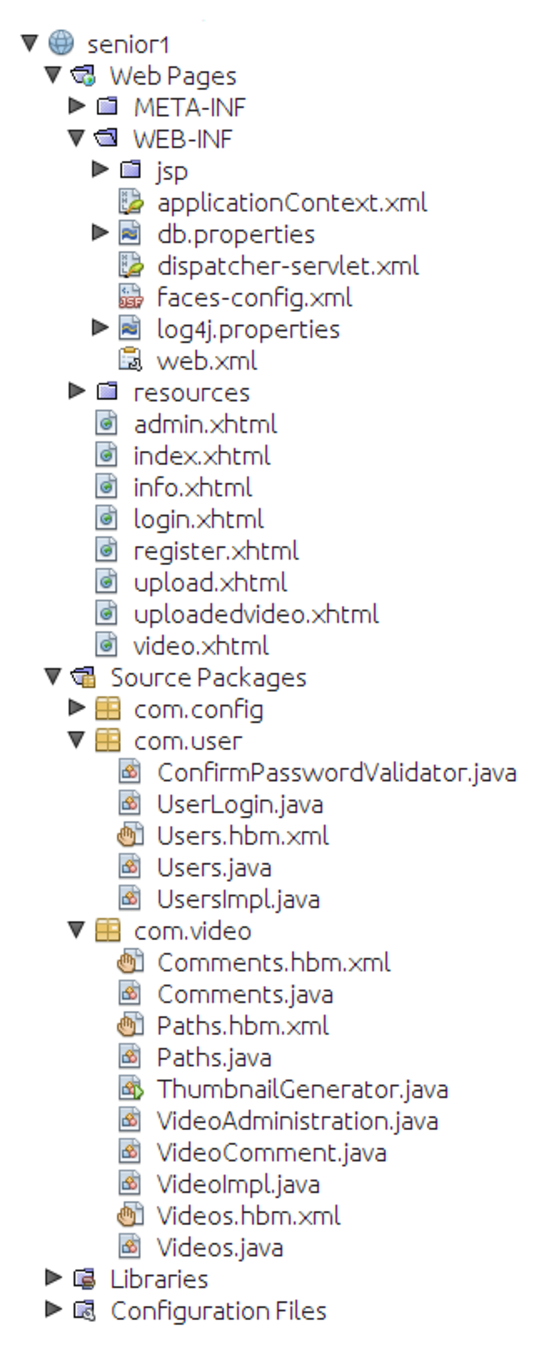
\includegraphics[scale=0.57]{picture/project_structure}}
	\end{center}
\end{figure}



\begin{algorithm}[H]
	\KwData{this text}
	\KwResult{how to write algorithm with \LaTeX2e }
	initialization\;
	\While{not at end of this document}{
	 read current\;
	 \eIf{understand}{
	  go to next section\;
	  current section becomes this one\;
	  }{
	  go back to the beginning of current section\;
	 }
	}
	\caption{\hl{Title of the Algorithm}}
\end{algorithm}


\newpage
\begin{code}
	\lstinputlisting[label=samplecode1,language=java, firstline=1, lastline=40]{project/src/java/com/user/UserLogin.java}
	\caption{\hl{Title of Code 1}}
\end{code}

\newpage
\begin{code}
	\lstinputlisting[label=samplecode2,language=xml]{project/src/java/com/user/Users.hbm.xml}
	\caption{\hl{Title of Code 2}}
\end{code}

\newpage
\begin{code}
	\lstinputlisting[label=samplecode3,language=html]{project/web/uploadedvideo.xhtml}
	\caption{\hl{Title of Code 3}}
\end{code}



\ac{ECC} is an acronym.






	\appendix\chapter{APPENDIX A:REQUIREMENTS SPECIFICATION DOCUMENT}
	\hl{Your Requirements Specifications Document (RSD v2.0) goes into this appendix.}

\hl{You can print it separately and append here.}



	\appendix\chapter{APPENDIX B: DESIGN SPECIFICATION DOCUMENT}
	\hl{Your Design Specifications Document (DSD v1.0) goes into this appendix.}

\hl{You can print it separately and append here.}



\end{document}
